\documentclass[a4paper]{scrartcl}

\usepackage{mathtools}
\usepackage{cleveref}
\usepackage{graphicx}
\usepackage{caption}
\usepackage{subcaption}
\usepackage{listings}
\usepackage[usenames,dvipsnames,svgnames]{xcolor}
\lstset{
    language=C++,
    basicstyle=\footnotesize\ttfamily,
    breaklines=true,
    keywordstyle=\color{DarkGreen}
    }
\DeclarePairedDelimiter\floor{\lfloor}{\rfloor}
\newcommand{\sse}{SSE}
\newcommand{\vec}[1]{\overrightarrow{#1}}

\author{Rico H\"auselmann}
\title{tinyvector}

\begin{document}
\maketitle
\section*{Introduction}
The \texttt{tinyvector} class template models a spin vector in the O(n) Model (a generalization of the Heisenberg Model). It's designed to hold a fixed, compile time known, number of numerical values.
The following mathematical operations are provided \cref{table:ops}. For some of them optimized versions for value type double are provided.

\begin{table}[h]
    \begin{tabular}{c l c r}
        Operation & function name & optimized & typical speedup\\
        $\vec{a} + \vec{b}$     & operator+ & yes & 1.3 \\
        $\vec{a} + x$           & operator+ & no & \\
        $\vec{a} - \vec{b}$     & operator- & yes & 1.3 \\
        $\vec{a} - x$           & operator- & no & \\
        $\vec{a} * \vec{b}$     & operator* & yes & 1.1 \\
        $\vec{a} * x$           & operator* & no & \\
        $\vec{a} / \vec{b}$     & operator/ & yes & 1.7 \\
        $\vec{a} / x$           & operator/ & no & \\
        $\text{sum}(\vec{a})$   & sum       & no & \\
        $\vec{a} \cdot \vec{b}$ & dot       & indirect & \\
        $\lvert\vec{a}\rvert$   & abs       & indirect & \\
    \end{tabular} 
    \caption{\label{table:ops}Operations provided by \texttt{tinyvector}. $*$ and $/$ are to be read as element-wise, $\cdot$ means dot product. Optimized versions are provided only for tinyvectors with value type double. The values in typical speedup are for a loop over $10^3$ operations for 4-dimensional vectors.}
\end{table}
%~ The \texttt{tinyvector} class template is intended to be used inside the inner loops of physics programs such as monte carlo spin simulations,
%~ inside the ALPS framework. Originally developed to hold spin vectors for the $O(n)$-Model it is designed for a very small amount of dimensions only
%~ as the runtime for such simulations scales exponentially in the number of dimensions.
%~ 
%~ Typically in the inner loop of the targeted kind of simulation not very complex operations are used on spin vectors; mostly addition, multiplication
%~ and dot products are applied. Thus, the four basic operations ($+, -, *, /$) were optimized using intrinsic vector instructions. 
%~ The optimized operations were benchmarked against the naive for loop implementation to see whether a speedup was obtained.

\section*{Usage}
\begin{lstlisting}
#include "tinyvector.hpp"

int main() {
    tinyvector<double, 3> vec1;                                // zero-initialized, optimizations disabled by default
    tinyvector<double, 4, NO_OPT> vec2 = {.25, .3, .1, 1.3};   // optimizations explicitly disabled
    tinyvector<double, 4, INTRIN_OPT> vec3;                    // zero-initialized, optimizations enabled
    tinyvector<double, 4, INTRIN_OPT> vec4 = {.1, .2, .3, .4}; // optimizations enabled

    auto a = vec2 + vec3;            // error
    auto b = vec3 + vec4;            // optimized

    tinyvector<int, 3, INTRIN_OPT> vec5;                        // no optimized specialization provided, fall back on non-optimized.
}
\end{lstlisting}

\section*{Implementation}
The class template \tinyvector is essentially a wrapper around a boost::array that takes an additional optimization tag template element and for which mathematical operations are defined.

\section*{Optimizations}
The optimized versions of the element-wise vector-vector operators call an intermediary template \texttt{\_vectorize} with a template argument to specify the operation.
The \texttt{\_vectorize} template recurses, at each recursion splitting off the right amount of elements to call the best available vector intrinsics operation with. The \texttt{\_vectorize} template specializations load the operands into vector registers where appropriate and then calls the operation type's static \texttt{apply} function.
Each operation type provides overloads for the apply function for elements as well as vector register pointers (\sse as well as AVX). This guarantees that the optimized version can fall back on the next level of vector instructions down to simple loop unrolling where \sse and/or AVX aren't available.

%\section*{OLDOPT}
%Optimization was only implemented on the level of individual \texttt{tinvyector}s. The applied methods are vectorization via intrinsics and complete loop unrolling, since it is intended for typically less than 16 elements. It will work for any number of elements in a \texttt{tinyvector}, however beyond a certain size complete loop unrolling is expected to become suboptimal.
%One of the \texttt{tinyvector}s template parameters, \texttt{Opt}, is used as a tag to determine wether optimization is desired by the user.
%The following operators are overloaded for \texttt{tinyvector<double, N, INTRIN\_OPT>} to use either AVX, SSE or simple kernels to minimize the number of operations needed for each \texttt{tinyvector}.
%The kernels and the associated dispatch mechanisms are contained within tinyvector\_kernels.cpp.
%
%\begin{lstlisting}
%template <int N>
%inline const tinyvector<double, N, INTRIN_OPT> & operator+=
%template <int N> 
%inline const tinyvector<double, N, INTRIN_OPT> & operator-=
%template <int N> 
%inline const tinyvector<double, N, INTRIN_OPT> & operator*=
%template <int N> 
%inline const tinyvector<double, N, INTRIN_OPT> & operator/=
%\end{lstlisting}
%
%The process of dispatching and chaining the calls to the most vectorized version of the basic operation for doubles will now be described using
%\texttt{operator+=} as an example.
%
%First the maximum amount of doubles on which will be operated simultaneously is stored in \texttt{STEP}.
%\begin{lstlisting}                                                                                                    
%/** 
% * determine the vectorization step length, aka how many doubles can we fit into a register? 
% */
%#ifdef __AVX__
%    const int STEP = 4;
%#else
%    #ifdef __SSE2__
%        const int STEP = 2;
%    #else
%        const int STEP = 1;
%    #endif
%#endif                                                                                                                  
%\end{lstlisting}
%
%The Operator struct \texttt{\_plus} defines \texttt{apply} functions for single values, vectors, SSE and AVX registers.
%Each just adds the \texttt{right} to the \texttt{left} argument in place.
%
%\begin{lstlisting}
%/**
% * operator kernels for different vectorization levels
% */
%struct _plus
%{
%    template <class T>
%    static inline const void apply(T & left, const T & right) {
%        left += right;
%    }
%    template <class vec>
%    static inline const void apply(vec & left, const vec & right, const int start) {
%        left[start] += right[start];
%    }
%#ifdef __SSE2__
%    static inline const __m128d apply(__m128d & mml, __m128d & mmr) {
%        return _mm_add_pd(mml, mmr);
%    }
%#endif
%#ifdef __AVX__
%    static inline const __m256d apply(__m256d & mml, __m256d & mmr) {
%        return _mm256_add_pd(mml, mmr);
%    }
%#endif
%};
%\end{lstlisting}
%
%The \texttt{\_vectorize} class template chains calls to its specializations, resulting in a completely unrolled sequence of 
%calls to \texttt{\_plus::apply} each using the best available vectorization (except for the remainder if $N \mod \texttt{STEP} \neq 0$, where the next best is used).
%
%\begin{lstlisting}
%/**
% * recursively call binary operator kernels 
% */
%template <class Op, int N>
%struct _vectorize {
%    template <class vec>
%    static inline const void apply(vec & left, const vec & right, const int start = 0) {
%        _vectorize<Op, STEP>::apply(left, right, start);
%        _vectorize<Op, N - STEP>::apply(left, right, start + STEP);
%    }
%};
%
%template <class Op>
%struct _vectorize<Op, 0>
%{
%    template <class vec>
%    static inline const void apply(vec & left, const vec & right, const int start = 0) { }
%};
%
%template <class Op>
%struct _vectorize<Op, 1>
%{
%    template <class vec>
%    static inline const void apply(vec & left, const vec & right, const int start = 0) {
%        Op::apply(left, right, start);
%    }
%};
%
%#ifdef __SSE2__
%
%template <class Op>
%struct _vectorize<Op, 2>
%{
%    template <class vec>
%    static inline const void apply(vec & left, const vec & right, const int start = 0) {
%        double * l = left.data();
%        const double * r = right.data();
%        __m128d mml, mmr, mms;
%        mml = _mm_load_pd(l + start);
%        mmr = _mm_load_pd(r + start);
%        mms = Op::apply(mml, mmr);
%        _mm_store_pd(l + start, mms);
%    }
%};
%
%#endif
%
%#ifdef __AVX__
%
%template <class Op>
%struct _vectorize<Op, 3>
%{
%    template <class vec>
%    static inline const void apply(vec & left, const vec & right, const int start = 0) {
%        _vectorize<Op, 2>::apply(left, right, start);
%        _vectorize<Op, 1>::apply(left, right, start + 2);
%    }
%};
%
%template <class Op>
%struct _vectorize<Op, 4>
%{
%    template <class vec>
%    static inline const void apply(vec & left, const vec & right, const int start = 0) {
%        double * l = left.data();
%        const double * r = right.data();
%        __m256d mml, mmr, mms;
%        mml = _mm256_load_pd(l + start);
%        mmr = _mm256_load_pd(r + start);
%        mms = Op::apply(mml, mmr);
%        _mm256_store_pd(l + start, mms);
%    }
%};
%
%#endif
%\end{lstlisting}  
%
%And finally the full definition for \texttt{operator+=}:
%
%\begin{lstlisting}
%/**
% * operator overload
% */
%template <int N>
%inline const tinyvector<double, N, INTRIN_OPT> & operator+= (tinyvector<double, N, INTRIN_OPT> & left, const tinyvector<double, N, INTRIN_OPT> & right) {
%    _vectorize<_plus, N>::apply(left, right);
%    return left;
%}
%\end{lstlisting}

\section*{Benchmarking}
The benchmark was written to be close to the use case, a class holding a \texttt{std::vector} of \texttt{tinyvector}s 
with a function that loops through the vector applying the operation to be benchmarked to every item in turn.
The runtime was measured in clock cycles using RDTSC.

The benchmarks were run on the EULER cluster. The compute nodes on EULER contain two 12-core Intel Xeon E5-2697v2 processors each with 32 KB of L1, 256KB of L2 and 2.5 MB of L3 cache per core.
All cores on this processor share L3 caches.

\section*{Results}
The Speedup of the optimized versus the naive default implementation for each of the four basic math operators was measured and plotted (\cref{fig:su-pl,fig:su-mi,fig:su-mu,fig:su-di}).

Typically for addition, subraction and multiplication speedups were in the range 0.5-1.5 for 2 and 3 dimensions, 1.0-2.0 for 4 dimensions and 1.2-4.5 for 16 dimensions depending on the number of \texttt{tinyvector}s processed in one iteration of the inner loop.
This suggests that for 2 and 3 dimensions some care should be taken to only use the optimized version of the tinyvector if the system size is greater than $10^3$ as for smaller systems it would be considerably slower. However in all other cases the optimized version should be at least about as fast as the naive implementation and potentially up to 5 times as fast.
Common to all three operators is a sharp reduction in speedup for the 16 dimensional \texttt{tinyvector} between system sizes $2^12$ and $2^13$.

For division on the other hand using the optimized version lead to significant speedups around 1.5-4.2 in allmost all cases, except for system sizes $2^17$ from $2^19$, where for 2-4 dimensions the speedup dropped to slightly below 1.0 and for 16 dimensions to about 2.0.

\begin{figure}
    \begin{subfigure}{\textwidth}
        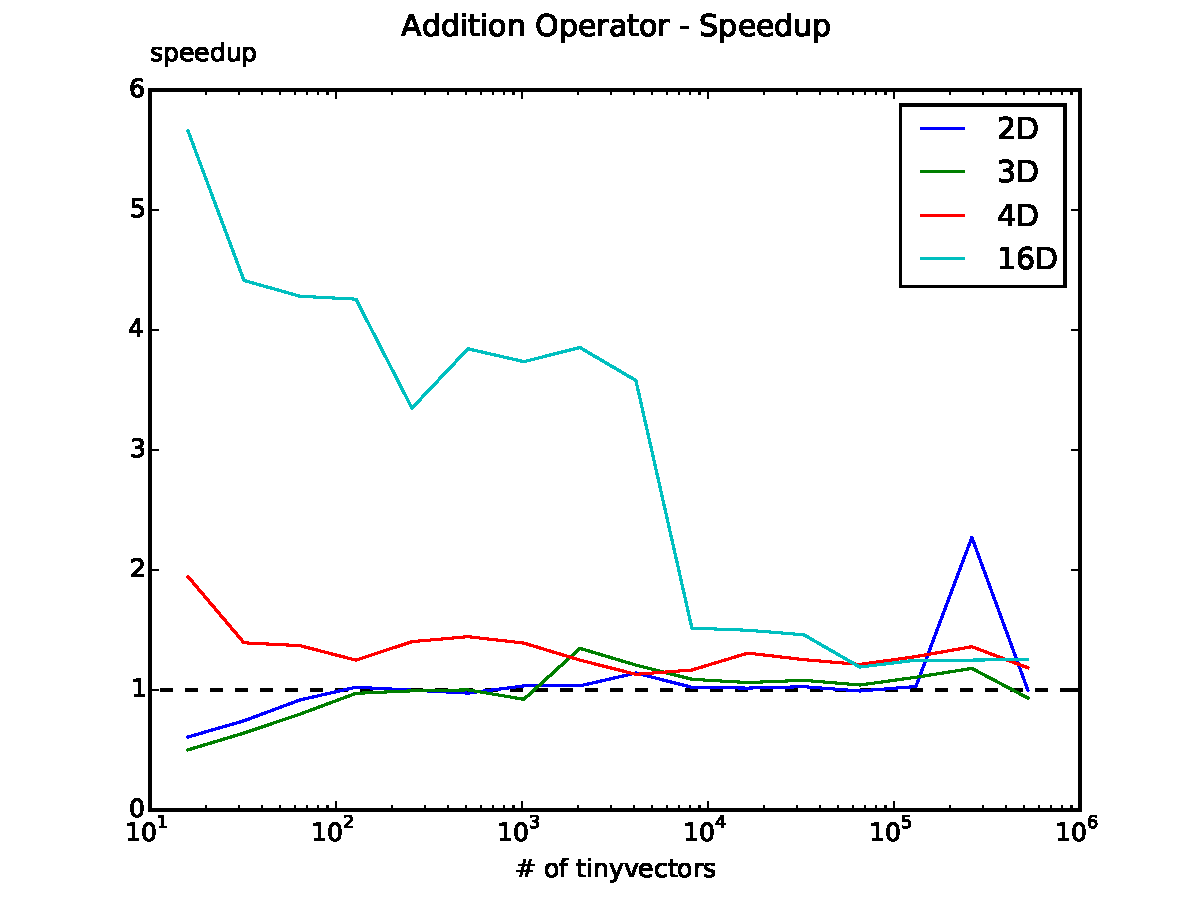
\includegraphics[width=0.8\textwidth]{results/su_plus.pdf}
        \caption{addition operator.}
        \label{fig:su-pl} 
    \end{subfigure}

    \begin{subfigure}{\textwidth}
        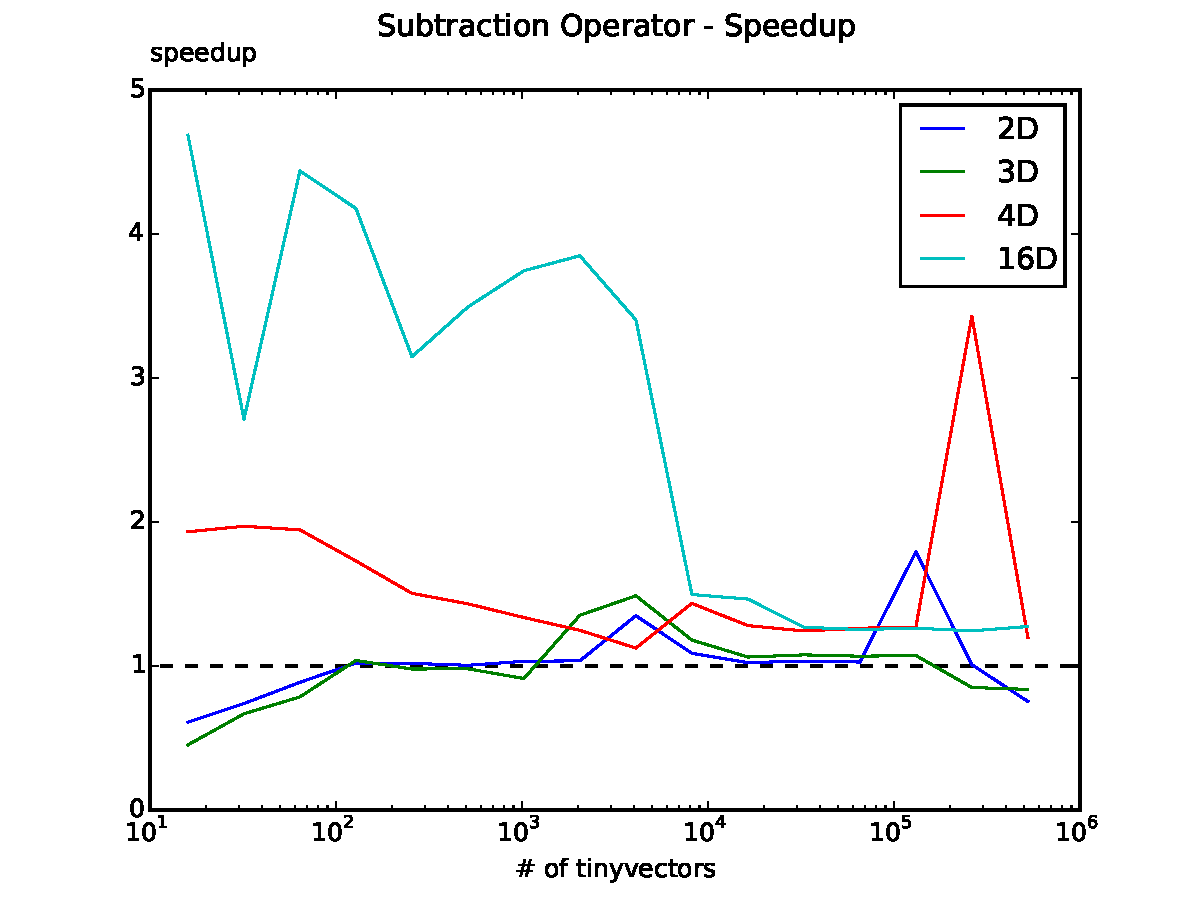
\includegraphics[width=0.8\textwidth]{results/su_minus.pdf}
        \caption{subtraction operator.}
        \label{fig:su-mi}
    \end{subfigure}
    \caption{Speedup of optimized vs. naive version for plus and minus operators for some tinyvector dimensionalities. \texttt{\# of tinyvectors} is the size of the \texttt{std::vector} containing the tinyvectors.}
\end{figure}

\begin{figure}
    \centering
    \begin{subfigure}{\textwidth}
        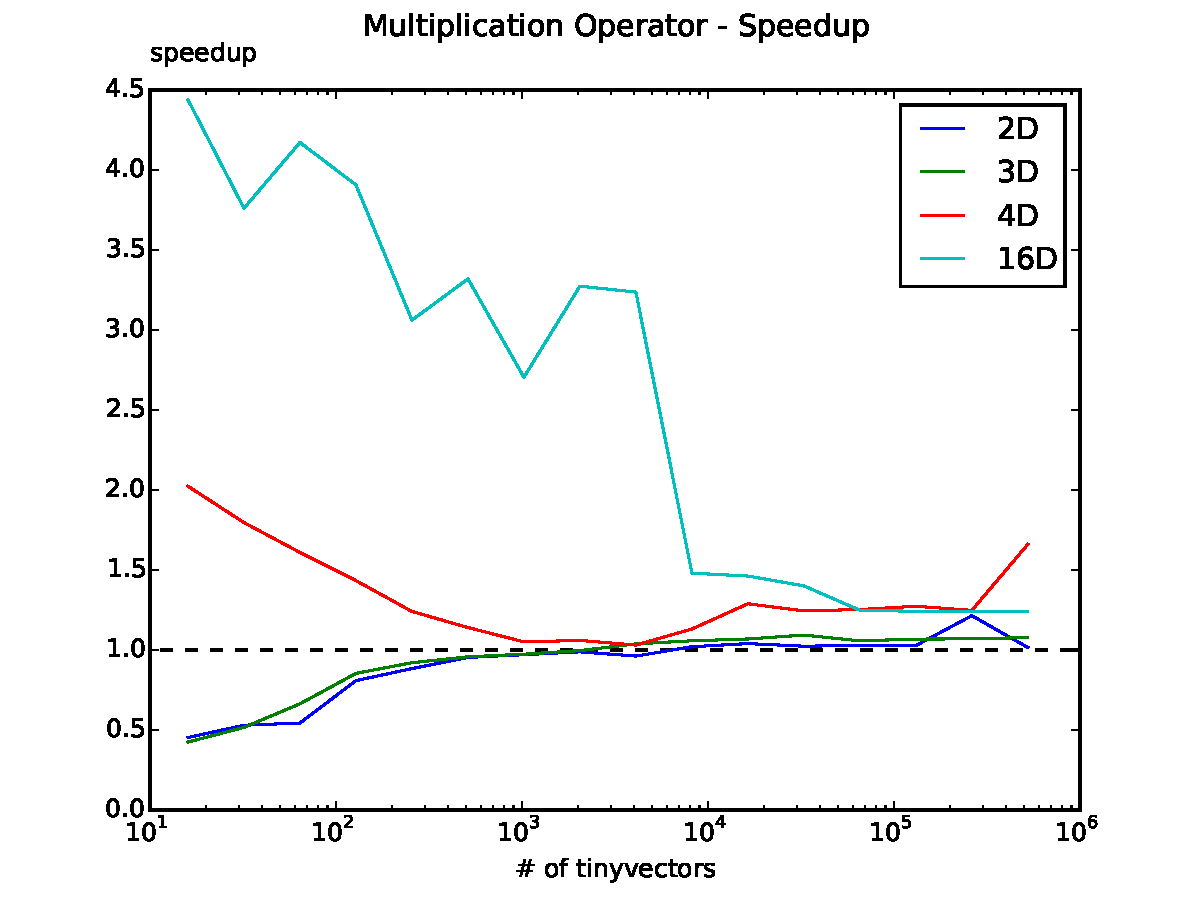
\includegraphics[width=0.8\textwidth]{results/su_multiply.pdf}
        \caption{(element wise) multiplication operator.}
        \label{fig:su-mu}
    \end{subfigure}

    \begin{subfigure}{\textwidth}
        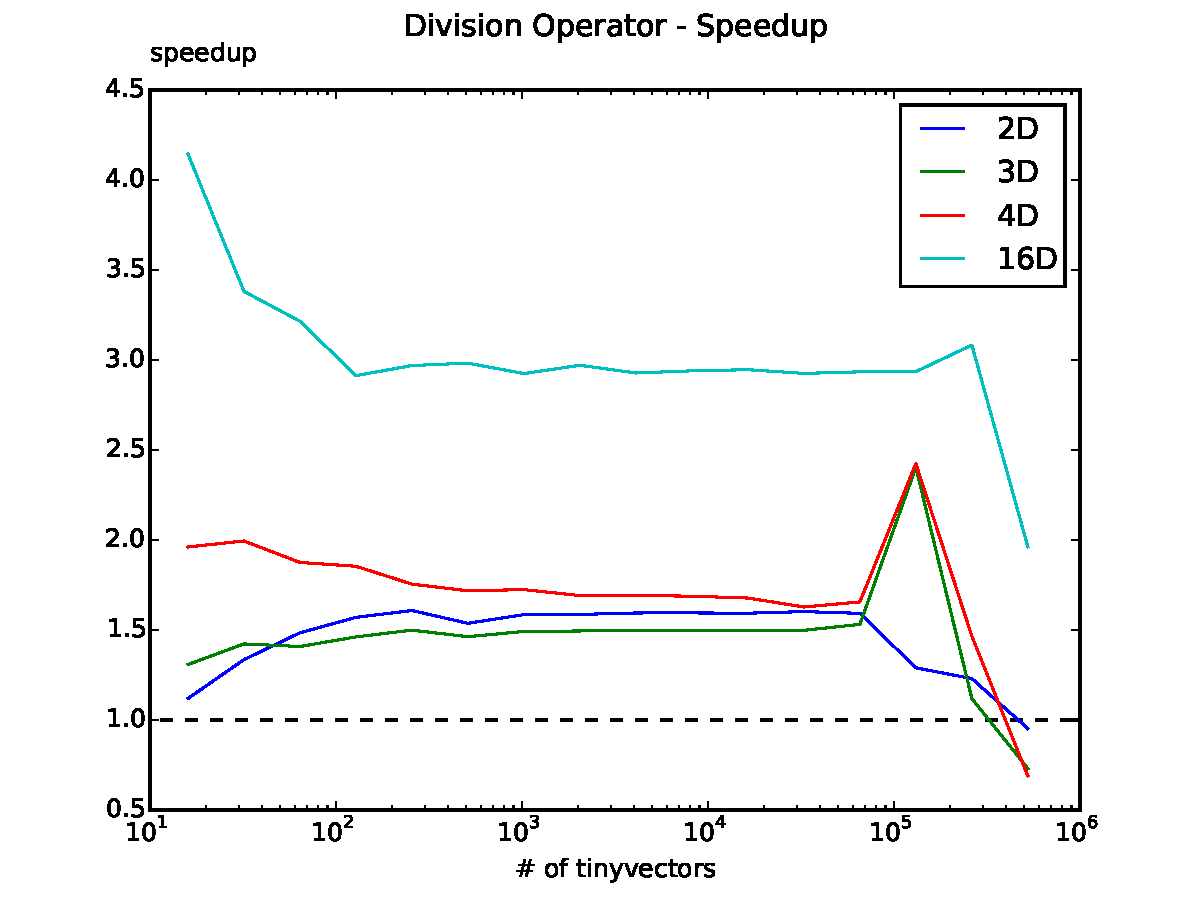
\includegraphics[width=0.8\textwidth]{results/su_divide.pdf}
        \caption{(element wise) division operator.}
        \label{fig:su-di}
    \end{subfigure}
    \caption{Speedup of optimized vs. naive version for multiplication and division operators for some tinyvector dimensionalities. \texttt{\# of tinyvectors} is the size of the \texttt{std::vector} containing the tinyvectors.}
\end{figure}

\end{document}
